% !TeX spellcheck = en_US
%% University of Groningen %% Faculty of Economics and Business %% Graduate School -SOM- 
%% Research Master in Economics and Business %% Research Master Thesis 
%% Student: Hugo Renato Vargas Aldana (s.2045427) 
%% Supervisor: Prof. Erik Dietzenbacher % 
%%%%%%%%%%%%%%%%%%%%%%%%%%%%%%%%%%%%%%%%%%%%%%%%%%%%%%%%%%%%% %------------------------------------------------------------

% Preamble

\documentclass[a4paper,12pt]{article} 
\usepackage{amsmath} 
\usepackage[spanish,english]{babel} 
\usepackage[applemac]{inputenc}
%\usepackage[ansinew]{inputenc} 
%\renewcommand{\baselinestretch}{1.5}
\usepackage[T1]{fontenc} 
\usepackage{natbib} 
\usepackage{amsfonts} 
\usepackage{amssymb}
%\usepackage{endnotes}
\usepackage{graphicx}
\usepackage{rotating}
\usepackage{longtable}
\usepackage[amssymb]{SIunits} 
\usepackage[margin=1.25in]{geometry}
\usepackage[font=small,labelfont=bf,tableposition=top]{caption}
\usepackage[official,right]{eurosym}
\usepackage{rotating}
\usepackage{subfigure}
\newtheorem{theorem}{Theorem}
\newtheorem{acknowledgement}[theorem]{Acknowledgement} 
\usepackage[colorlinks=true,linkcolor=blue,citecolor=black,urlcolor=blue]{hyperref}
%\parindent0em


%\makeindex


% RM-THESIS
\begin{document} 

\bibliographystyle{apa-good}

\title{Economies to die for: Impacts on human health embodied in production and trade\thanks{An earlier version of this paper was submitted as research master thesis of the main author at the University of Groningen.}} 
\author{Renato Vargas\thanks{Instituto de Agricultura, Recursos Naturales y Ambiente, Rafael Landivar University \mbox{(renovargas@gmail.com)}.} \\ Erik Dietzenbacher\thanks{Faculty of Economics and Business, University of Groningen.}} 

%\date{August, 2012.} 
\date{March, 2015.} 

\maketitle

\begin{abstract} 
Using an extended input-output model of 41 regions, this study evaluates impacts on human health embodied in production and trade. The input-output methodology is used in a similar manner as done in environmental studies related to ecological footprints. The study covers deaths attributable to pollution and payments made to the health industry by economic activities. These measures are assessed when output is delivered to satisfy final demands locally and abroad. Findings show that Bulgaria, China, Indonesia, India, Latvia, Romania, Russia, and the Rest of the World are net producers of fatalities embodied in trade. It can be said that these regions save their trade partners from having to deteriorate the health of their citizens. Conversely, industries with highest levels of payments to the health sector per direct and indirect unit of output intended for final demand are mostly located in the developed world, with the clear exception of China, whose heavy industries appear to be making large investments in human capital per unit of output. 

%In this study I assess the notion that countries that transfer part of their industrial production abroad avoid the ill effects of said production when human health externalities are also moved overseas. I evaluate the responsibility regarding human health costs that the local consumption of a country causes globally. % An emphasis is placed on the US economy. (Think if this is necessary. Maybe not.)
%I proxy the human health cost embedded in production and trade in three ways. First, I link US economic consumption to global direct and indirect expenditures on local health sectors in a world input-output model. Second, I establish the on-the-job injuries and missed work days embedded in trade with selected partners of the US. Finally, I examine the direct and indirect health costs paid in the form of health insurance premiums by employers in the US and assess the avoided costs of moving production overseas by individual sector of that country.
\end{abstract}



\section{Introduction}

%Arouse interest, present research question and introduce the sections of the paper. Although, this paper is of an exploratory nature, one of the underlying motivations behind it is connected to the ``pollution haven hypothesis''. This hypothesis tries to explain that as societies in developed nations bec

This study explores the distribution of impacts of economic activity on human health around the world using input--output analysis. Although this methodology has been used extensively for the assessment of environmental impacts embedded in trade (see \citealp{wiedmannexamining2007}, for a review), its application to human health mostly has been undertaken in an indirect way. An adaptation of a multi-regional input--output model has been carried out here, in order to understand the more direct relationship between production, trade, and human health. The twofold question that this adaptation tries to answer is: \textbf{``How does global trade relate to local health quality and how is the responsibility for health impacts distributed globally?''}

Section \ref{sec:bg} presents a brief review of the literature of input--output studies related to trade and the environment, from which the intuition for the methodology used here is taken. Also, relevant literature that looks into the link between pollution and health is evaluated. An explanation of the pollution haven hypothesis and how it might play a role in this kind of studies is also provided, even if this study does not explicitly set out to prove or disprove its theoretical underpinnings. Section \ref{sec:method} presents a basic input--output model, which is then expanded to a multi--region model that takes the link between human health and production into account. It also explains the variables related to human health used in this study. Section \ref{sec:results} presents the results and a final section provides a conclusion.


\section{Background}
\label{sec:bg}

%Literature review goes here (make link to the pollution haven hypothesis and present literature that argues that some countries might be exporting their externalities, and hence their ``on-the-job'' health risks as well. The classic example is that of the iPhone factory workers that get intoxicated with heavy metals). Keep to the point.



The notion of assessing the embodied content of health related variables in products and trade resembles that carried out in environmental studies of responsibility or ``footprint'' analyses---that is, evaluating to what degree a country extends its impacts on this earth across its borders. In this study an attempt is made to view human health under a similar light as the term \textit{virtual water} \citep{allanvirtual2003} or the more broad ``ecological footprint'' \citep{reesrevisiting1996,wackernagelour1996}, which reflects the total land needed by a country, in order to absorb the impact of its residents on the planet.

In the particular case developed here, that means that imports allow an economy with less tolerance to human health deterioration to escape the stress of negatively affecting the health of its inhabitants. The degree to which it can do so is given by a factor determined by the higher tolerance to health deterioration of its trade partners. From this, it follows that it is possible to the global distribution of health impacts embedded in trade that are caused when local output is delivered in order to satisfy demands home and abroad.

As explained above, there is an established tradition of input-output literature that has undertaken these types of analysis for environmental variables \citep{wiedmannexamining2007}. Some focus, not only on the accounting of environmental impacts embodied in trade, but also on the discussion of how to assign responsibility for them to consumers that buy products that come from abroad \citep{steengeinputoutput1999,munksgaardco22001,gallegoconsistent2005,rodriguesdesigning2006,lenzenshared2007,rodriguesconsumer2008}. 

A preferred topic, due to the the special interest on climate change and the international agreements derived to address it, seems to be that of the emission content of imports and exports. Many of these studies focus on specific countries, such as India 
\citep{dietzenbacherempirical2007}, Italy \citep{mongelliglobal2006}, Denmark \citep{munksgaardco22001}, or Spain  
\citep{sanchezcholizco22004,serranodietz2010}, and a few take a bilateral approach (\citealp{rheechange2006}, \citealp{ackermancarbon2007}, or \citealp{normaneconomic2007}, for example). However, multi-regional studies can assess these global relationships of impacts of trade and responsibility allocation in a way that can provide better insights \citep{wiedmannallocating2006,turnerexamining2007}.

The limitation behind conducting such multi--regional studies lays in the availability of input-output data for many regions. Nevertheless, important contributions have been made. For example, \citet{peterspost-kyoto2008} analyzed CO$_2$ emissions embodied in international trade for 87 regions. \citet{weberembodied2007} also analyzed the trade environmental relationships between the US and seven of its trade partners, and \citet{ahmadcarbon2003} estimated the emissions embodied in international trade of goods of over 20 regions/countries. For this study, use is made of the World Input-Output Datatabase (WIOD)\footnote{Available at \url{http://www.wiod.org}.}, which provides input-output matrices for 27 European countries, 13 other relevant world economies, and the rest of the world.

Literature regarding the link between health and pollution is also extensive, although not commonly related to input-output studies. \citet{cohenurban2004} and \citet{ostro2004outdoor} offer some of the most comprehensive evidence for the effect of pollution on human burden of disease, as well as its assessment for international comparison. Their work serves as empirical backing for the \textit{deaths attributable to pollution} measure used in this study\footnote{See section \ref{subsec:polludeath}.}. Notwithstanding, most of the literature concerning this link is done at the country level, due to the fact that impacts of different sources of pollution on health are a highly geographically localized issue. \citet{zuidemahealth1997}, for example, have investigated the link between work loss days for the labor population and average yearly concentrations of air pollution in 29 districts in the Netherlands, finding a significant relationship between pollutants and morbidity. Similarly, \citet{khannameasuring2000} has developed an index of pollution based on the dose-response of each pollutant and certain types of welfare loss for the US. \citet{cifuenteseconomic1993}, on the other hand, have estimated the marginal benefits of air-pollution abatement due to health effects also in the US, considering a damage function. 

\citet{mukhopadhyayforsell2005} have claimed a more actual and concrete linear link between impacts on health and emissions from fuel combustion and have brought impacts on health into the realm of input-output studies. This has provided the structural analysis literature with an advance from so-called \textit{impacts caused} (emissions) to \textit{impacts borne} (health impacts). They essentially found out that, for the case of India, changes in air pollution and health impacts can be explained by changes in the same structural factors (pollution intensity, technology, and final demand). The present study aims to contribute to that line of work.

On the other hand, assessing the link between economic activity, pollution, and human health links this exercise to the pollution haven hypothesis, even if it is not the intention here to test it. This hypothesis posits that trade allows countries to move away from producing environmentally sensitive activities (in terms of natural resources, pollution, and, from the explanation above, health impacts).

This situation can be interpreted from the Heckscher-Ohlin model of trade, where an increase in trade will lead countries to specialize in industries where they enjoy a comparative advantage. The Heckscher-Ohlin model describes this advantage from the relative abundance of either labor or capital regarding another country. It predicts that the relatively labor abundant country will export the good that is produced relatively labor intensive and will import the relatively capital intensive good. Later efforts have extended the scope of analysis to include other factors, such as natural resources (see \citealp{leamerleontief1980,leamersources1985}; or \citealp{bowenmulticountry1987}). For those extensions, in a world with two countries and two goods, each country would  specialize in the good for which  the natural resource intensity relative to the other country's is the least.

A similar extension can be made regarding the measures for embedded health impacts used in this study, due to the link with environmental quality. The implication is that if the pollution haven hypothesis is true, developing countries will produce more ``unhealthy'' commodities---those high in embedded health impacts---than their trade counterparts in developed countries. At the same time they will meet their final demand of more ``healthy'' products---low on embedded health impacts---via imports from developed nations. The opposite can be said from the latter.

This can happen because of different reasons. For example, it can be assumed that developed countries that have populations with higher incomes and firmly established institutions will demand better working conditions and health coverage systems, as well as better environmental controls. On the contrary, developing countries, with lower levels of income are thought to place a higher value on \textit{any} jobs that can be generated, with less concern over the negative impacts that could accompany them. Accordingly, it can be assumed that in developing countries, controls for overall environmental quality and health will be lax.

In the context of the Heckscher-Ohlin model, these assumptions translate into developing countries being abundant in an intangible factor that can be thought of (in a somewhat draconian fashion) as the extent to which they are willing to deteriorate the health of their inhabitants.  Developed countries, will be less abundant in this factor due to labor protection laws, collective agreements, and stronger environmental controls. It follows that developing countries will specialize in commodities whose production poses larger threats to human health, while developed nations will do so in the opposite type of commodities.

In essence, all this would happen for economic reasons through an indirect mechanism that would represent elevated costs for business owners in more health conscious nations (where compliance with environmental and human safety regulations is costly) making it attractive to locate or relocate production to countries with lax controls. As a consequence, trade will exacerbate existing health problems in those developing countries with relatively lax environmental and social security regulations. 

As a counterargument, it has been argued that findings for these type of studies can also be interpreted from the factor endowments hypothesis \citep{dietzenbacherempirical2007}. These authors explain that pollution intensities of production are highly correlated with capital intensities, and thus capital-abundant nations (generally from the developed world) have a comparative advantage in pollution intensive goods. If the links that were established in this introduction between production, environment, and human health are accurate, it could also happen that developed nations would also specialize in goods high on embodied health impacts. This would happen simply because they are abundant in capital and heavy industry has more impacts to the environment and hence human health.

Finally, \textit{payments to the health sector}---one of the variables evaluated here---can be thought of as an investment in human capital and counteracting force against health deterioration. For example, \citet{fangGavazza2011} interpret such payments, when made by employers in a mixed public-private health care system, as a factor. They take the viewpoint that health is a general form of human capital that affects workers' productivities on the job. Then, higher investments in human capital from developed nations would make them more abundant in this factor and thus more likely to specialize in ``healthy'' commodities. The opposite would be true to developing nations.

%Cite \citet{muradiantrade2001}.


\section{Methodology}
\label{sec:method}

In this section the basic input-output model is presented and expanded in order to assess human health impacts in a multi-regional context. The number of deaths attributable to pollution\footnote{''Deaths attributable to pollution'' and ``deaths'' are used interchangeably.}---one of the measures---is used to explain the basic elements of the calculations and in later sections a generalization is made. 
%These injuries are entered in the model in the form of a set of coefficients that explain their incidence per unit of production.
A second measure is based on expenditures from all sectors in all countries to their respective health sector.

\subsection{Model}
\subsubsection[]{Basic input-output model} 
\label{sec:basicio}

Throughout this paper, economic relationships of interest are presented in the form of an input-output model. The economy is comprised of $e$ economic industries or sectors, which produce an output that may be used by themselves or other sectors as an input, or by final users (e.g. households, the government, etc.) as consumption, investment, or gross exports. Regions are thought to differ in the technology they use to produce. For that reason, different production ``recipes'' apply for a unit of a certain sector's
output, depending on its origin.

The economy's interindustry inputs are given by the matrix $\mathbf{Z}=[z_{ij}]$, which identifies purchases of industry $i$'s output by industry $j$. A vector $\mathbf{f}=[f_j]$ defines the sales of sector $j$ to final demand elements, and a vector $\mathbf{x}=[x_j]$ gives total output of industry $j$. Put together for individual industries, the relationship between these elements can be expressed as

\begin{equation} 
x_j=z_{j1}+\cdots+z_{je}+f_j.
\label{01} 
\end{equation} 

Stacking the equations for individual sectors, the same relationship can be expressed in matrix notation\footnote{Traditionally, in input-output studies bold, upright capital letters denote matrices, upright lower case letters, vectors, and italicized lower case letters, scalars. A diagonal matrix with a vector on its main diagonal and zeros elsewhere is denoted by an upright lower case letter with a circumflex ( $\mathbf{\hat{}}$ ). See \citet{miller2009}, \textit{Appendix A}, for an introduction to input-output notation.} as

\begin{equation}
\mathbf{x = Zi + f}, \label{02} 
\end{equation}

\noindent where $\mathbf{i}$ is a summation vector of ones and length $e$. Consequently, direct input coefficients (input per dollar of output) can be defined as
$\mathbf{A}=[a_{ij} = z_{ij}/x_j]$, which in matrix form reads

\begin{equation} 
\mathbf{A = Z\hat{x}^{-1}}. 
\label{03} 
\end{equation}


From (\ref{02}) and (\ref{03}), the entire system can be expressed more generally as

\begin{equation} 
\mathbf{x = Ax+f}, 
\label{04} 
\end{equation}

\noindent and rearranged results in

\begin{equation} 
\mathbf{(I-A)x = f}. 
\label{05} 
\end{equation}

\noindent Finally, if changes in demand are simulated, the new output can be estimated by solving (\ref{05}) for $\textbf{x}$

\begin{equation} 
\mathbf{x = (I-A)^{-1}f=Lf}, 
\label{06} 
\end{equation}

\noindent where $\mathbf{(I-A)^{-1}=L=}[l_{ij}]$ is known as the \textit{Leontief inverse} or the \textit{total requirements matrix}. Its values represent the additional direct and indirect production in $i$ that has to be realized in order to meet an additional unit of final demand of product $j$.

\subsubsection[Multi-regional model]{Extension of the basic model to a multi-regional model and assessment of the health sector}
\label{sec:mregmod}

The approach described in this section expands the basic model to a multi-regional input-output model, in order to compute an international balance of injuries at the workplace between regions. The methodology is fashioned after a similar approach used to assess the responsibility of a country in regard to emissions, with some conceptual adjustments (See \citealp{serranodietz2010}, for a useful comparison of global responsibility evaluation methods). The coefficient of deaths per unit of output is used as
an approximation of the local health deterioration embedded in goods and services that are traded locally and globally. 

%\footnote{Draft Note: Ask Erik about thecomparability of measures between countries, since IMF exchange rates were used on the WIOD.} 

The extension of equation (\ref{06}) to a multi-country approach is straightforward when interpreting the matrices explained in section \ref{sec:basicio} as a collection of regional matrices. In matrix notation, the arrangement of those regions in the input-output model, expanding on (\ref{04}), is represented by the partitioned structure where $r,s=\{1,\ldots,n\}$ are selling and purchasing industries, respectively, and

\begin{equation} 
\left( \begin{array}{c} 
\mathbf{x^1} \\ 
\vdots\\ 
\mathbf{x^n}\\ 
\end{array} \right) = 
\begin{bmatrix}
\begin{array}{ccc} 
\mathbf{A^{11}} & \ldots & \mathbf{A^{1n}} \\ 
\vdots &  \ddots &  \\ \mathbf{A^{n1}} &  & \mathbf{A^{nn}}
\end{array} 
\end{bmatrix} 
\left( \begin{array}{c} \mathbf{x^1} \\ \vdots\\ \mathbf{x^n}\\ \end{array} \right) + \left(
\begin{array}{c} \mathbf{f^{11}} +  \ldots  +  \mathbf{f^{1n}} \\ \vdots  \\ \mathbf{f^{n1}}  +  \ldots  +  \mathbf{f^{nn}}
\end{array} 
\right) 
\label{07} .
\end{equation}

An important conceptual difference exists between the individual region and the multi-regional model. For the individual region model, all interregional\footnote{``Interregional'' is to be interpreted as ``intercountry''.} trade is given exogenously as part of the final demand ($\mathbf{f}$) in the form of exports, regardless of their use in the final destination. In the multi-region model, however, trade is given by purchases between industries from different regions and interregional final demand purchases. 

For that reason, the partitioned matrix ($\mathbf{A}$) above is composed of regional matrices ($\mathbf{A}=\begin{bmatrix}
\begin{smallmatrix} \mathbf{A^{11}}&\mathbf{A^{1n}}\\ \mathbf{A^{n1}}&\mathbf{A^{nn}} \end{smallmatrix} \end{bmatrix}$). Its individual element ($\mathbf{A} = [a^{\mathbf{rr}}_{ij}]$) denotes interregional trade relationships when ($r \not= s$)---the off-diagonal elements---, and intrarregional trade when ($r=s$)---elements in the main diagonal. Final demands ($\mathbf{f^{rr}}$), has to be noted, contains deliveries to final consumers, non-profit organizations serving households, the government, gross fixed capital formation, and changes in inventory.

A vector of coefficients $\mathbf{c^{e \times n}}$, equivalent to $[c^r_{j}=h^r_j/x^r_j]$, is constructed to incorporate the health perspective, where $c$ identifies the number of deaths $h$ 
%\footnote{Draft Note: Originally, I had followed a previous approach used in a multi-year projection of GHG emissions. There, I used a matrix of coefficients $[\mathbf{C^r}=c^r_{kj} ]$, where $k$ stood for each of the different GHGs, that when premultiplied by the model it returned economy-wide total emissions of individual pollutants. That was done analogously in this study at first, anticipating that, for health issues there would be various ways of making expenses comparable internationally (e.g. per worker, as a percentage of total value added, as a percentage of GDP...), as well as various measures of health impacts, such as injuries and fatalities at the workplace or insurance premiums paid per worker. However, in order to assess responsibilities of 1435 sectors worldwide, the single number yielded by that model was not practical because that meant that tailor-made equations would have to be crafted for each of the 41 regions, in order to compute either producer responsibilities, consumer responsabilities, or health impacts embedded in trade, from individual matrix or vector components. Therefore, a different approach was formulated in order to create a matrix where individual stakeholders' responsibilties (of sectors or regions) were evident and easily computed by indexed system-wide equations. That could only be achieved mantaining disagreggation of the calculation components, and thus a single impact measure vector ($\mathbf{c}$) was to be used at a time. It is turned into a diagonal matrix ($\mathbf{\hat{c}}$) and postmultiplied by the model, where ($\mathbf{f}$) is also entered as a diagonal matrix ($\mathbf{\hat{f}}$), yielding matrices on which indexed results can be more readily calculated.} 
generated per unit of output $x$ of sector $j$ in region $r$. Total deaths ($h$) generated in all regions is defined by

\begin{equation} 
%\begin{pmatrix} 
%\begin{array}{c} 
%\mathbf{h^1} \\ 
%\vdots\\ 
%\mathbf{h^r}\\ 
%\end{array} 
%\end{pmatrix} 
%=
%\left( 
%\begin{array}{c} 
%\mathbf{C^1 x^1} \\ 
%\vdots  \\ 
%\mathbf{C^r x^r} 
%\end{array}
%\right). 
\mathbf{h = \hat{c}x} 
\label{08}
\end{equation}

\noindent Since it is known from (\ref{06}) that $\mathbf{x = Lf}$, then in patitioned form

\begin{equation} \begin{pmatrix} \begin{array}{c} \mathbf{h^1} \\ \vdots\\ \mathbf{h^n}\\ \end{array} \end{pmatrix} =
\begin{bmatrix} \begin{array}{ccc} \mathbf{\hat{c}^1 L^{11}} & \ldots & \mathbf{\hat{c}^1 L^{1n}} \\ \vdots &  \ddots &  \\ \mathbf{\hat{c}^n L^{n1}}
&  & \mathbf{\hat{c}^r L^{nn}} \end{array} \end{bmatrix} \left( \begin{array}{c} \mathbf{f^{11}} +  \ldots  +  \mathbf{f^{1n}} \\ \vdots 
\\ \mathbf{f^{n1}}  +  \ldots  +  \mathbf{f^{nn}} \end{array} \right). \label{09} 
\end{equation}

%The multiplication of the coefficient vector ($\mathbf{c}$) with the Leontief inverse ($\mathbf{L}$) yields a vector of coefficients that translate final demands into direct and indirect totals of the health measure under evaluation. Further multiplication by the regional final demands added into one vector ($\mathbf{f}$) yields a single number of the system-wide total health measure ($h$). However, in order to assess the responsibilities of the different stakeholders (sectors, final demands, and regions) without having to resort to cumbersome partitioned notation, it is important to keep the individual elements disaggregated. That can be accomplished with resources from matrix multiplication rules and their notation conventions. (Erik thinks this is true but superfluous.)
In order to maintain disaggregation, the coefficient vector is turned into a diagonal matrix ($\mathbf{\hat{c}}$). It then premultiplies ($\mathbf{L}$), which yields a matrix $\mathbf{H}=[h^{rs}_{ij}]$. Its elements identify the extra deaths in sector $i$ of region $r$ that implicitly take place when an extra unit of goods or services from sector $j$ is needed to satisfy final demands
in region $s$. Thus,

\begin{equation} \begin{pmatrix} \begin{array}{c} \mathbf{h^1} \\ \vdots\\ \mathbf{h^n}\\ \end{array} \end{pmatrix} =\begin{bmatrix}
\begin{array}{ccc} \mathbf{H^{11}} & \ldots & \mathbf{H^{1n}} \\ \vdots &  \ddots &  \\ \mathbf{H^{n1}} &  & \mathbf{H^{nn}}
\end{array} \end{bmatrix} \left( \begin{array}{c} \mathbf{f^{11}} +  \ldots  +  \mathbf{f^{1n}} \\ \vdots  \\ \mathbf{f^{n1}}  + 
\ldots  +  \mathbf{f^{nn}} \end{array} \right).
\label{10}
\end{equation}

Matrix ($\mathbf{H}=\mathbf{\hat{c}L}$) is interesting in itself, because it readily shows which sectors in which regions have the highest (or lowest) number of deaths per unit of final demand; or simply \textit{health impact multipliers}. Since levels are important, however%and responsibility is not only attributed to the producer, but also to those who trigger that production
, a final procedure (equation \ref{11} below) yields a mechanism to identify a net balance between stakeholders. First, if the individual regional final demand vectors from the last part of equation (\ref{10}) are known, instead of summing into a single vector, a matrix ($\mathbf{F}
%=\begin{bmatrix} \begin{smallmatrix} \mathbf{f^{11}}&\mathbf{f^{1s}}\\ \mathbf{f^{r1}}&\mathbf{f^{rs}} \end{smallmatrix} \end{bmatrix}
$) can be constructed from them.
Postmultiplication of  ($\mathbf{H}$)  with said matrix will yield a nonsquare final demand responsibility matrix ($\mathbf{G}$) of dimensions ($ne \times n$) as a collection of vectors ($\mathbf{g}$). The column sums correspond to the  responsibilities of the final demand of each region in regard to the health measure at hand. The vector of its row sums of is equal to $\mathbf{h}$. In matrix notation, this is $\mathbf{G}= \mathbf{\hat{c}LF}$. Partitioned, it reads 

\begin{equation} \begin{bmatrix} \begin{array}{ccc} \mathbf{G^{11}} & \ldots & \mathbf{G^{1n}} \\ \vdots &  \ddots &  \\
\mathbf{G^{n1}} &  & \mathbf{G^{nn}} \end{array} \end{bmatrix} = \begin{bmatrix} \begin{array}{ccc} \mathbf{H^{11}} & \ldots &
\mathbf{H^{1n}} \\ \vdots &  \ddots &  \\ \mathbf{H^{n1}} &  & \mathbf{H^{nn}} \end{array} \end{bmatrix} \begin{bmatrix}
\begin{array}{ccc} \mathbf{f^{11}} & \ldots & \mathbf{f^{1n}} \\ \vdots &  \ddots &  \\ \mathbf{f^{n1}} &  & \mathbf{f^{nn}}
\end{array} \end{bmatrix} . \label{11} \end{equation}

The row sums  of matrix $\textbf{G}$ identify the deaths embodied in deliveries from each industry in every region needed to satisfy final demands home and abroad. Column sums, in turn, represent total deaths embodied in purchases from industries in all regions to meet individual region's final demands. Additionally, if the matrix is aggregated at the country level on its rows, then it becomes square. The off diagonal elements ($\textbf{g}^{\textbf{rs}}$ when $r \not= s$) of this aggregated matrix represent the exports of deaths from region $r$ to region $s$ (i.e. deaths in region $r$ that are embodied in the final demand of region $s$).

\begin{equation}\text{\textit{Net balance of deaths for country} $r$} = \sum_s g^{rs} - \sum_s g^{sr}. \label{12} \end{equation}

Finally, the percentage structure of each column can be interpreted as the shares of origin of imported deaths for every country. The percentage structure of each row, alternatively, denotes the shares of destination of deaths for every country.

\subsection{Human health impact measures and coefficients}
\label{sec:vars}

In order to better understand how economic regions interact with human health in the multiregional input-output model, the \textit{coefficient of deaths per unit of output} $\mathbf{c^r}=[c^r_{j}=h^r_j/x^r_j]$ explained in section \ref{sec:mregmod} is extended conceptually to reflect another measure (to substitute for $h^r_j$). In practice, this translates into separate
exercises being conducted for: 1) deaths attributable to outdoor air pollution per unit of output, and 2) payments to the health sector of a given region per unit of output. These measures differ in the degree to which they can be considered good proxies for the relationship between human health and the economy and the kind of questions that they can answer. 
%and they are ordered in no particular order other than comprehensiveness of the data (as explained in section \ref{sec:data}).

%A detailed explanation follows.

\subsubsection{Deaths attributable to outdoor air pollution} \label{subsec:polludeath}

This set of coefficients (in place of $\mathbf{c}=[c_{j}=h_j/x_j]$ above) uses the burden of disease resulting from exposure to urban outdoor air pollution to substitute for $h$. Specifically for this study, burden of disease refers to deaths that are brought about by a complex mixture of air pollutants emitted by industrial activities and households, of which fine particulate matter has the greatest effect on human health \citep{cohenurban2004}.

Evidence from epidemiological studies have shown that exposure to urban air pollution is linked to three diseases in an important manner, among others \citep{ostro2004outdoor}. These are respiratory infections in children under 5 years of age,  as well as cardiopulmonary disease and lung cancer in adults over 30. The measure links the incidence of deaths from these diseases to air quality in urban centers worldwide.

A more detailed explanation of the indicator can be found in appendix \ref{appendix:classif}, but in essence, its calculation is done by combining information on the increased risk of a disease resulting from exposure to fine particulate matter with information of the spread of this exposure in cities. From this a fraction is derived that gives the total number of deaths from urban pollution when applied to the total incidence of the diseases mentioned above \citep*{who2012}.

The information is collected and estimated by the Global Health Observatory of the World Health Organization and the unit of measurement is the number of deaths in a given year. For this study, this measure provides a direct link between the environment and the health of populations around the world. Since industrial production is a strong contributing factor to the quality of air in cities, an indirect link can be assumed to exist between the WIOD model and this variable. However, as stated above, quality of air is also influenced by households, so not all of the deaths attributable to pollution can be linked to economic industries. To correct for this situation, the number of deaths is reduced using the share of the production of total greenhouse gas emissions that corresponds only to economic industries for every region\footnote{The input-output system presupposes linear relationships between its different matrices, vectors, and even the individual elements that form these. That is why it is possible to use the share of pollution of industries to correct the number of deaths directly, even if levels of pollution are not explicitly used within the model. This is mathematically equivalent to reducing the amount of pollutants to those generated by industries alone, and then multiplying them by a coefficient of deaths per ton of pollutant. Both reductions (of pollutants and deaths) would be in the same proportion.}.

It can be expected that developing countries will be more abundant in a factor that reflects their implicit willingness to risk human lives for the creation of jobs. Hence, costs associated with maintaining good health will be lower. The opposite will be true of developed countries. Hence, developing countries will specialize in ``fatal'' commodities and will import ``non-fatal'' commodities to satisfy their final demand from developed countries. This will reflect a positive balance of deaths due attributable to pollution embodied in exports less deaths in imports for this class of nations.


%\subsubsection{Occupational injuries}
%\label{subsec:injuries}
%
%The first set of coefficients is created using occupational injuries at the workplace in place of $h^r_j$ explained above. Member countries of the International Labour Organization aim to collect data on occupational injuries by economic activity\footnote{Following the \textit{Resolution concerning statistics of occupational injuries} resulting from occupational accidents, available at: \newline \url{http://laborsta.ilo.org/applv8/data/SSM8/E/ANNEX.html}.}, with different degrees of success regarding detail and comprehensiveness. ILO has compiled this information within its Laborsta project for various years. The measure is constructed in a straightforward way by recording the cases of one worker incurring an occupational injury as a result of one occupational accident in a specific economic sector\footnote{See appendix \ref{appendix:classif} for details.}.
%
%This measure provides a link between workforce health and economic sectors in the different regions. 
%
%Using this measure has the positive aspect that, for the most part, data on injuries is collected by national health statistics systems, which in turn use medical records and household surveys for their construction. This fact indicates that the sub-reporting that could be expected from employers is avoided. 
%% Thus, the degree to which this variable is a valid proxy for overall health is improved. 
%
%However, there are issues to consider. Even if this health metric is directly related to production, its unit of measurement refers to highly visible cases and does not account those that never make it to the hospital (or to treatment). Unhealthy working conditions may contribute to chronic illnesses (skin conditions, respiratory illnesses, cancer, and others) that presumably are not captured with this variable. Furthermore, the data that is available for this variable is difficult to compare internationally due to different definitions used by member nations and different levels of coverage. For example, while the US has disaggregated information for nine industrial sectors, China only offers a grand total for some state-owned enterprises. Without efforts of data reconciliation and harmonization, results cannot be conclusive. Time constraints allow this variable to be used as an exploratory reference resource only.



\subsubsection{Payments to the health sector of a given region per unit of output}
\label{subsec:payhealth}

As implied in section \ref{sec:basicio}, an individual column of the direct requirements matrix ($\textbf{Z}$) represents the purchases that a given economic sector makes to itself and other industries home or abroad---the ``recipe'' to create its output. Of those entries, the purchases that industries make to the \textit{Health and Social Work} industry\footnote{Here, the ``\textit{Health and Social Work} sector'', ``the health sector'', and ``the health industry'' are used interchangeably.} are considered a reasonable candidate to link industry output to direct and indirect human health costs of production in this study. The scope of said industry is given by
the International Standard Industrial Classification of All Economic Activities (ISIC) and it is explained in detail in appendix \ref{appendix:classif}. The advantage of this indicator is that the information describing it is harmonized within the World Input-Output Database (WIOD) and it is comprehensive for the period covered by it (1995-2009).

Essentially, the health sector represents five clusters of activity. First, it quantifies the activities of general and specialized hospitals and other health institutions with accommodation facilities. These activities are directed to in-patients mainly and they are carried out under supervision of medical doctors. Second, it includes the consultation and treatment activities of general physicians and medical specialists including dentists, either at private practices or in clinics such as those attached to firms and other institutions. Third, it assesses those activities related to human health not performed by doctors or dentists, like optometry and occupational therapy, which may be conducted in the same private practices or clinics as the second category. Fourth, it describes the economic activities of orphanages, correctional facilities, homes for the elderly and such. Lastly, the health sector within the input-output system also takes into account activities of veterinary hospitals, veterinarians in the field, such as in farms, and other health services for animals provided by veterinary assistants.

%\begin{table}[!hbtp] %	\caption{Description of the contents of the Health and Social Work Sector} %\begin{center} 
% \includegraphics[width=5in]{somegraphicnamewithoutfileextension} 
%\centering 
%\textbf{\textit{Element about here.}} 
%\end{center}
%	\label{tab01} %\end{table}

Due to the above, purchases to the \textit{Health and Social Work} sector represent actual health related services that can be linked to economic activity. Conversely, purchases to other related fields, like the \textit{Defence and Compulsory Social Security} sector or the \textit{Financial Intermediation}\footnote{In the case of private insurance.} sector, represent social security benefits or insurance services whose medical component may or may not be realized during the accounting period. Moreover, mandatory contributions to social security do not necessarily (have to) correlate with medical services rendered. 
% % They have more to do with the size of the welfare state.

Nevertheless, a link with health can only be assumed when sectors purchase either of the first three components of the health sector explained previously (hospitals, clinics, and therapists) and not when the values refer to the last two (permanent institutions such as orphanages, or veterinary services). Since the actual shares spent on each category are not possible to disaggregate from the World Input-Output Model data, the study is conducted with the help of simplifying assumptions.

In the case of institutions like orphanages and correctional facilities, the assumption is made that governments, through the \textit{Public Administration} activity, are most likely to be the ones purchasing these kinds of services. Thus, recorded payments to the health sector made by other industries refers only to health services. 
%Furthermore, an assumption is made regarding the scope of the government to be limited to a region, preventing final demands from other countries to buy these institutional services indirectly through governmental exports. 
This study also assumes that no veterinary services are purchased by the industries considered, except for the health sector itself that probably subcontracts to itself part of the veterinarian services demanded from it, and the agricultural sector\footnote{\textit{Agriculture, Hunting, Forestry and Fishing}.}, which presumably purchases a large share of veterinary services. To circumvent these issues, adjustment factors reduce the values of health purchases made by these three industries.

One of those factors reduces the agricultural sector's purchases of health to a lower level (15\% of the original value), a second one reduces the health sector's purchases of own production to three quarters of the total value (75\%), and a third one does the same for the \textit{Public Administration} activity. It is recognized that this is done in an arbitrary manner in the face of data constrains. Further investigation can correct this situation by disaggregating National Accounts data for every country of the WIOD database.

In sum, it is assumed that firms that purchase from the health sector actually need medical services for their employees. In an exploratory manner, this variable is expected to provide insights regarding the global distribution of health costs.



\newpage
%\section{Data} \label{sec:data}
%
%\subsection{World Input-Output Database (WIOD)}
%
%The WIOD 1995-2009 tables form a model of the world economy that consists of 27 countries from the European Union and 13 other major
%countries, developed in order to ``analyse the effects of globalization on trade patterns, environmental pressures and
%socio-economic development across a wide set of countries'' (European Commission). In essence, it is an input-output model that
%consists of 40 regions and one ``rest of the world,'' where each region differs in production technology. Inside each region, there
%are $35$ sectors...
%
%\subsection{ILO - Laborsta Database}
%
%Describe the database from the International labor Organization.
%
%\subsection{WHO - Global Health Observatory Data}
% 
%Describe the WHO - GHO data.

\section{Results}
\label{sec:results}

%In this section, focus is placed on producer versus final demand responsibilities regarding health impacts, health impact intensities, and health impacts embodied in trade. Although figures and tables are kept concise here for presentation purposes, more comprehensive results can be found in appendix \ref{appendix:results}.
In the previous sections a basic input-output model was extended in order to obtain a multi-regional model with which to assess the global distribution of direct and indirect impacts on human health triggered by economic activity. In this section, results from these calculations are presented. First, focus is placed on deaths attributable to pollution embodied in products. Afterwards, payments to the health sector are assessed in a similar manner. 

%\subsection{Occupational Injuries}
%
%The first measure assessed in the study identifies the distribution of injuries sustained at the workplace around the world. With the help of the adapted model from section \ref{sec:method}, responsibility for direct and indirect injuries embedded in output was determined. Due to the fact that the data for various countries has not been harmonized, results included can only serve as test of the methodology and reference.
%
%Table \ref{tab01a} shows the average intensity of occupational injuries---direct and indirect per \$US billion of output destined for final demand home and abroad. In the top quintil, Portugal, Germany, Spain, Slovenia, Mexico, Malta, and France can be found as the places with most injuries per unit of output. On the other hand, the bottom quintil is dominated by Greece, Latvia, Japan, China, Romania, Ireland, and India. 
%
%\begin{table} %[!hbtp] 
%\caption{Average Intensity of Occupational Injuries (\textit{direct and indirect injuries per \$US billion of output}) -- Year 2008} 
%\begin{center}
%\small \begin{tabular}{lrlr}
% & \textbf{Average} &  & \textbf{Average} \\ 
%\textbf{Region} & \textbf{Intensity }& \textbf{Region} & \textbf{Intensity}\\ 
%\hline
%Portugal &  16,087  & Hungary &  3,022 \\ 
%Germany &  15,301  & Slovakia &  2,551 \\ 
%Spain &  14,879  & Luxembourg &  2,503 \\ 
%Slovenia &  14,635  & Great Britain &  2,354 \\ 
%Mexico &  11,167  & Cyprus &  1,972 \\ 
%Malta &  8,867  & Austria &  1,900 \\ 
%France &  8,557  & Bulgaria &  1,671 \\ 
%Italy &  7,663  & Netherlands &  1,606 \\ 
%Czech Republic &  6,984  & Sweden &  1,505 \\ 
%Australia &  6,107  & Russia &  1,487 \\ 
%Brazil &  5,644  & Lithuania &  1,417 \\ 
%Finland &  5,417  & Greece &  1,104 \\ 
%Poland &  4,916  & Latvia &  1,040 \\ 
%Canada &  4,597  & Japan &  734 \\ 
%Belgium &  4,481  & China &  659 \\ 
%Rest of the world &  3,802  & Romania &  564 \\ 
%Denmark &  3,463  & Ireland &  531 \\ 
%United States &  3,231  & India &  100 \\ 
%Estonia &  3,099  &  & \\
%\hline
%\end{tabular}
%\label{tab01a} 
%\end{center}
%\end{table}
% 
% In general, the results of this measure appear to follow no intuitive pattern, but this is thought to be an issue of data reconciliation and harmonization. The other two measures show international relationships that seem more intuitive in the realm of global distribution of health impacts and their responsibilities. Attention is directed at payments to the health sector and deaths due to pollution embedded in trade.

\subsection{Deaths attributable to pollution embedded in output}

The first measure assessed in the study identifies the distribution of deaths attributable to pollution around the world. With the help of the adapted model from section \ref{sec:method},  deaths embodied in output destined for final demand were determined. This measure provides an intuitive link between the global distribution of production and human health. %More payments to the health sector, not necessarily could be interpreted as a more deteriorated health. However, 
Deaths due to pollution are a clear indicator of the negative externalities that production has on the countries where it is located. In this section, results are presented for the year 2008.

Data for deaths attributable to pollution is only available at the national level. For that reason results cannot be disaggregated at the sector level, and furthermore, Taiwan had to be aggregated into China and Malta had to be aggregated into the rest of the world region. Table \ref{tab04} provides average multiplier ($r^\text{\textit{th}}$ row sum of matrix H, divided by the number of countries) for each of the regions analyzed, sorted from highest to lowest. The top quintil of direct and indirect deaths due to pollution per billion dollars of output destined for final demand is occupied by China (336), India (284), the Rest of the World (217), Russia (157), Bulgaria (152), Indonesia (97), and Romania (70).



\begin{table} [!hbtp] 
\caption{Average Multiplier of Deaths Due to Pollution (\textit{deaths embodied output needed to satisfy an additional \$US million of final demand}) -- Year 2008} 
\begin{center}
\small \begin{tabular}{lrlr}
 & \textbf{Average} &  & \textbf{Average} \\ 
\textbf{Region} & \textbf{Multiplier}& \textbf{Region} & \textbf{Multiplier}\\ 
\hline
China & 336 & United States & 14\\ 
India & 284 & Czech Republic & 13\\ 
Rest of the world & 217 & Germany & 12\\ 
Russia & 157 & Japan & 12\\ 
Bulgaria & 152 & Italy & 12\\ 
Indonesia & 97 & Spain & 10\\ 
Romania & 70 & Slovakia & 9\\ 
Turkey & 66 & Netherlands & 7\\ 
Latvia & 58 & Australia & 7\\ 
Brazil & 31 & France & 6\\ 
Poland & 28 & Denmark & 6\\ 
South Korea & 25 & Slovenia & 5\\ 
Mexico & 25 & Belgium & 5\\ 
Lithuania & 24 & Sweden & 5\\ 
Portugal & 22 & Finland & 5\\ 
Hungary & 22 & Canada & 3\\ 
Greece & 21 & Austria & 3\\ 
Estonia & 17 & Ireland & 1\\ 
Cyprus & 16 & Luxembourg & 0\\ 
Great Britain & 15 &  &  \\
\hline
\end{tabular}
\label{tab04} 
\end{center}
\end{table}

On the other end of the distribution, the bottom quintil is dominated by Belgium (5), Sweden (5), Finland (5), Canada (3), Austria (3), Ireland (1), and Luxembourg, with a (0.2), which in terms of deaths is the equivalent as having no deaths per billion dollars worth of direct and indirect output delivered to final demand.

The top quintil is interesting in the sense that it includes some of the countries that traditionally have been thought of having lax environmental regulations and have attracted polluting industries, such as China, India, and Russia. However, while the intensity of health impact (deaths due to pollution per \$US billion of direct and indirect output needed to satisfy final demand) provides a clear point of comparison between countries, the country's impact on global human health can only be properly assessed when compared with the level of production, the origin of the deaths delivered to a country embedded in trade, and the destination of a country's embedded deaths.

Matrix ($\mathbf{G}$) from equation (\ref{11}) provides such information when its rows are aggregated to the country level. As explained in section \ref{sec:method}, its off diagonal elements correspond to trade of embedded deaths between regions. Table \ref{tab05} shows deaths embodied in exports, imports and a balance for the year 2008. It shows that for that year, Bulgaria, China, Indonesia, India, Latvia, Romania, Russia, and the Rest of the world are net producers of fatalities embodied in trade. It can be said that these regions save the rest from having to deteriorate some of the health from their citizens.

\begin{table} %[!hbtp] 
\caption{Deaths embodied in exports, imports, and balance -- Year 2008} 
\begin{center}
\small \begin{tabular}{lrrr}
 & \textbf{Deaths in} & \textbf{Deaths in} &  \\ 
\textbf{Region} & \textbf{Exports}& \textbf{Imports} & \textbf{Balance}\\ 
\hline
Austria &  236  &  6,222  & (5,986)\\ 
Australia &  469  &  2,221  & (1,752)\\ 
Belgium &  586  &  3,420  & (2,834)\\ 
Bulgaria &  1,634  &  589  & 1,045 \\ 
Brazil &  2,497  &  5,214  & (2,717)\\ 
Canada &  598  &  7,857  & (7,259)\\ 
China &  159,071  &  20,348  & 138,723 \\ 
Cyprus &  26  &  223  & (197)\\ 
Czech Republic &  686  &  1,729  & (1,043)\\ 
Germany &  3,462  &  20,716  & (17,254)\\ 
Denmark &  349  &  1,864  & (1,515)\\ 
Spain &  1,175  &  8,767  & (7,592)\\ 
Estonia &  77  &  206  & (129)\\ 
Finland &  193  &  1,737  & (1,544)\\ 
France &  1,130  &  12,330  & (11,200)\\ 
Great Britain &  2,480  &  13,040  & (10,560)\\ 
Greece &  457  &  2,151  & (1,694)\\ 
Hungary &  882  &  1,250  & (368)\\ 
Indonesia &  5,150  &  3,610  & 1,540 \\ 
India &  26,218  &  8,327  & 17,891 \\ 
Ireland &  64  &  1,591  & (1,527)\\ 
Italy &  1,942  &  11,210  & (9,268)\\ 
Japan &  3,177  &  24,713  & (21,536)\\ 
South Korea &  4,105  &  10,743  & (6,638)\\ 
Lithuania &  208  &  504  & (296)\\ 
Luxembourg &  4  &  255  & (251)\\ 
Latvia &  267  &  224  & 43 \\ 
Mexico &  2,630  &  4,941  & (2,311)\\ 
Netherlands &  1,034  &  6,155  & (5,121)\\ 
Poland &  1,860  &  3,352  & (1,492)\\ 
Portugal &  590  &  1,196  & (606)\\ 
Romania &  1,546  &  1,357  & 189 \\ 
Russia &  15,618  &  7,092  & 8,526 \\ 
Slovakia &  235  &  899  & (664)\\ 
Slovenia &  63  &  422  & (359)\\ 
Sweden &  373  &  2,521  & (2,148)\\ 
Turkey &  3,421  &  4,471  & (1,050)\\ 
United States &  4,823  &  65,483  & (60,660)\\ 
Rest of the World &  89,785  &  70,171  & 19,614   \\
\hline 
Total & 339,121 & 339,121 & 0 \\
\hline
\end{tabular}
\label{tab05} 
\end{center}
\end{table}

That those eight economic regions can be considered pollution havens comes from the fact that the deaths embedded in their exports are more numerous than the deaths embedded in their imports. However, that does not imply that the rest of regions do not export deaths. Matrix ($\mathbf{G}$) from equation (\ref{11}) allows us to identify the origin (rows) and destination (columns) of the embodied deaths in trade. Figure \ref{fig01} shows a stylized version of this\footnote{Abbreviations: AUS (Austria), AUT (Australia), BEL (Belgium), BGR (Bulgaria), BRA (Brazil), CAN (Canada), CHN (China), CYP (Cyprus), CZE (Czech Republic), DEU (Germany), DNK (Denmark), ESP (Spain), EST (Estonia), FIN (Finland), FRA (France), GBR (Great Britain), GRC (Greece), HUN (Hungary, IDN (Indonesia), IND (India), IRL (Ireland), ITA (Italy), JPN (Japan), KOR (South Korea), LTU (Lithuania), LUX (Luxembourg), LVA (Latvia), MEX (Mexico), MLT (Malta), NLD (Netherlands), POL (Poland), PRT (Portugal), ROM (Romania), RUS (Russia), SVK (Slovakia), SVN (Slovenia), SWE (Sweden), TUR (Turkey), TWN (Taiwan), USA (United States), ROW (Rest of the World).}. In part \ref{fig01a}, the percentage structure was calculated for the columns, and then the diagonal (corresponding to local transactions) was removed. This structure corresponds to the shares of origins of deaths embodied in trade for every region. A gray scale identifies the larger origins with darker tones. Part \ref{fig01b} was done in a similar fashion. However, in this case the percentage structure was calculated for the rows, identifying the destinations of deaths embodied in trade for every region. Higher percentages in the destinations are marked with darker tones, as well.

Visual examination of these two figures shows some trends in the form of darker horizontal or vertical lines. The darker horizontals in \ref{fig01a} identify countries that are important origins of the direct and indirect deaths embodied in trade. This is the case of China, India, Russia, and the Rest of the World, followed by a faint Germany, Indonesia, and Romania.

The darker verticals in \ref{fig01b} identify countries that are important destinations for the direct and indirect deaths embodied in trade intended for final demand. In this case, Germany, France, Great Britain, Italy, the United States, and the Rest of the world are clear destinations, followed by China and Spain.


\begin{figure}
\centering
\subfigure[Origin of deaths embodied in trade (relative structure of matrix~$\textbf{G}$'s columns from eq.~\ref{11} with hidden own purchases in diagonal).]
{
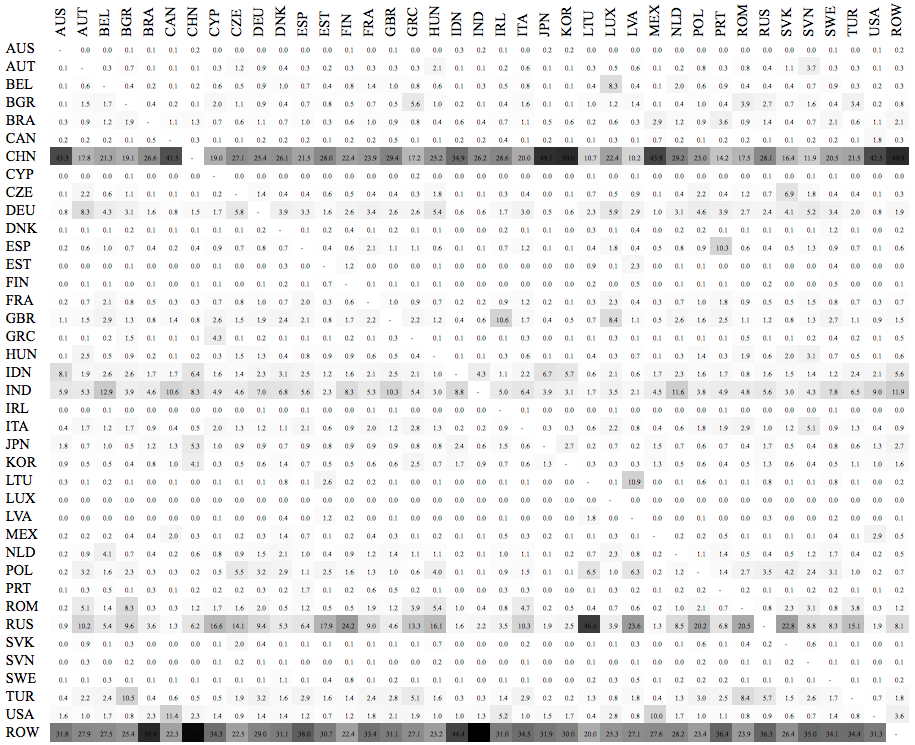
\includegraphics[width=4.5in]{origin}
\label{fig01a}
}
\\
\subfigure[Destination of deaths embodied in trade (relative structure of matrix~$\textbf{G}$'s rows from eq.~\ref{11} with hidden own purchases in diagonal).]
{
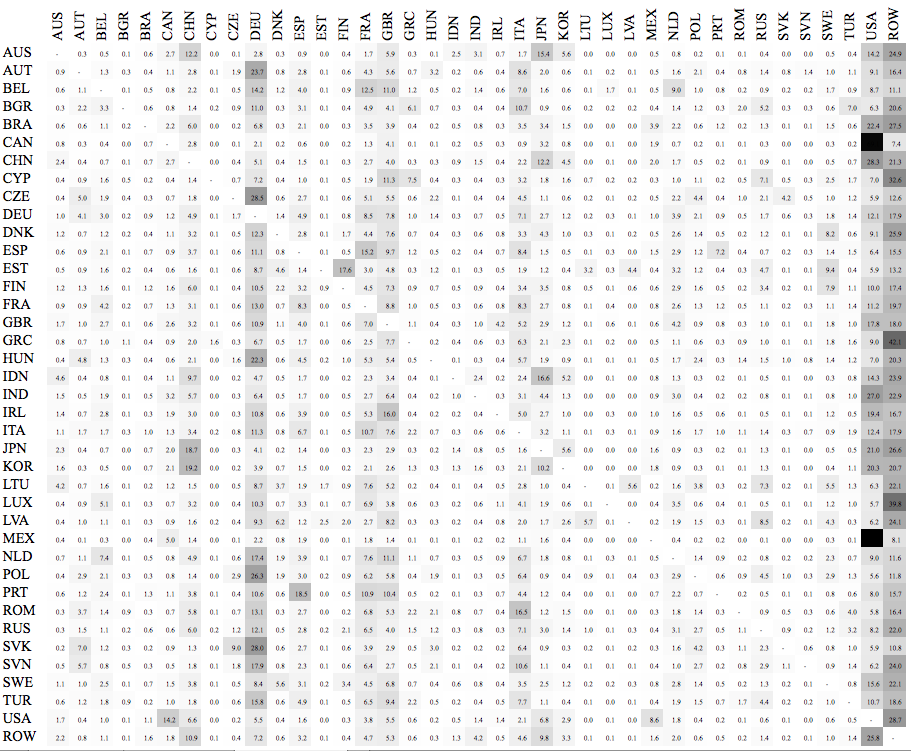
\includegraphics[width=4.5in]{destination}
\label{fig01b}
}
\caption{Origin and Destination of deaths embodied in trade -- Year 2008}
\label{fig01}
\end{figure}


\subsection{Payments to the Health and Social Work Industry}

All sectors in every region may make purchases to their respective health sector. From the World Input--Output Database the direct payments can be read straightaway for each year of the period 1995--2009, showing the distribution of the employer-paid health care around globally. With help of the model explained in section \ref{sec:method}, it has been possible to capture the indirect payments to the health industry that are made worldwide when final demands for all regions are met\footnote{The year 2008 is used for several items of this discussion, for presentation purposes, but information for more years was estimated and can be found in appendix \ref{appendix:results}.}.

Matrix $\mathbf{H}$ from equation (\ref{10})---when calculated for this health measure---provided multipliers for each of the 1435 production industries considered in the WIOD\footnote{35 industries $\times$ 41 regions.}, related to the deliveries for final demand to each of the 41 regions. For comparison, \textit{average multipliers} were estimated as row averages of that matrix. These refer to the average deaths embodied in the delivery of one unit from one country to each of its trade partners. Table \ref{tab01} shows the results for the 30 sectors with the highest average payments to the health sector that were made per \$US million delivered to final demand in the year 2008\footnote{30 are shown for space considerations and explanatory purposes. They correspond to 2\% of the cases for that year. The same calculations have been conducted for all years of the 1995--2009 period. The \textit{Health and Social Work} industry of all regions has been removed from this ranking, due to its overwhelming multiplier size, which comes from extensive purchases to itself, presumably in the form of subcontracting. Table \ref{tab02} shows an aggregate of that industry.}.  

The first element that draws attention is that this table is headed by the public administration and social security sector of Canada, which triggered the payment of \$US107.1 in health services for every million dollars of output that were delivered to final demand home or abroad in 2008. The reasons behind this disproportionate number in relation to the rest of the list deserves attention. This can be explained due to a high interconnectedness of this sector with industries that pay extensively to the health sector (home and abroad), as well as to the acclaimed universal public health coverage of Canada.

\begin{table} %[!hbtp] 
\caption{30 industries with highest average multiplier and their regions (\textit{\$US of payments to health industry per \$US million of output intended for final demand}) -- Year~2008} 
\begin{center}
\small \begin{tabular}{llr}
  &  & \textbf{Average}\\ 
 \textbf{Industry} & \textbf{Region} & \textbf{Multiplier}\\ 
 \hline
Public Adm. and Defence; Social Security & Canada & 107.1\\ 
Mining and Quarrying & Rest of the world & 43.8\\ 
Basic Metals and Fabricated Metal & China & 27.5\\ 
Electrical and Optical Equipment & China & 26.0\\ 
Machinery & China & 25.7\\ 
Mining and Quarrying & China & 24.9\\ 
Financial Intermediation & Great Britain & 20.2\\ 
Education & Canada & 16.5\\ 
Transport Equipment & China & 16.0\\ 
Renting of Machinery and Equipment & France & 15.8\\ 
Renting of Machinery and Equipment & Spain & 15.3\\ 
Chemicals and Chemical Products & China & 14.7\\ 
Electricity, Gas and Water Supply & China & 13.6\\ 
Renting of Machinery and Equipment & Sweden & 10.3\\ 
Wholesale Trade and Commission Trade & Spain & 10.0\\ 
Renting of Machinery and Equipment & Netherlands & 9.5\\ 
Renting of Machinery and Equipment & Denmark & 9.1\\ 
Renting of Machinery and Equipment & China & 9.0\\ 
Renting of Machinery and Equipment & Rest of the world & 8.8\\ 
Retail Trade & Taiwan & 8.5\\ 
Renting of Machinery and Equipment & India & 8.4\\ 
Other Services & Malta & 8.3\\ 
Other Non-Metallic Mineral & China & 8.1\\ 
Chemicals and Chemical Products & Great Britain & 7.9\\ 
Pulp and Paper & China & 7.7\\ 
Chemicals and Chemical Products & Austria & 7.6\\ 
Other Services & France & 7.2\\ 
Renting of Machinery and Equipment & Great Britain & 7.2\\ 
Financial Intermediation & Greece & 7.1\\ 
Post and Telecommunications & Spain & 6.7\\ 
\hline
\end{tabular}
\label{tab01} 
\end{center}
\end{table}

A second feature of interest of table \ref{tab01} relates to the fact that it is dominated by Chinese heavy industry: Basic Metals and Fabricated Metal, \$US27.5; Electrical and Optical Equipment, \$US26.0; Machinery, \$US25.7; Mining and Quarrying, \$US24.9; Transport Equipment, \$US16.0; Chemicals and Chemical Products, \$14.7; Other Non-Metallic Mineral \$US8.1; Pulp and Paper, \$US7.7, per million dollars of output intended for final demand. Here, this is presumed to be explained by the amount of the world's production that has been relocated to China over the past decades and its sheer size. Most of the Chinese industries in the list correspond to sectors that are traditionally capital intensive, but that can easily be argued that make heavy use of the abundant labor in that country, and hence are related to extensive payments to the health sector per unit of output there. It has to be emphasized that the intensity described here refers, not only to direct payments made by these sectors, but also to payments made by all sectors related to them directly and indirectly via inputs in the production process. 

It is also noteworthy that the \textit{Mining and Quarrying} industry of the Rest of the World is positioned as second highest in the list (\$US43.8 per million dollars of output intended for final demand). 
%If the assumptions made here are correct, high payments to the health sector per unit of output mean a poorer health condition of the workforce directly and indirectly related to the sector in question. 
The World Input-Output Database has a strong emphasis on the European economy and other prominent countries in the world economy\footnote{27 EU countries and 13 other economies in addition to the Rest of the World.}. This means that very few of the lower end of the developing economies are featured explicitly in it and get lumped together in the Rest of the World region.

The role of less developed countries in the production of raw materials, especially minerals, has been a traditional topic of interest in international economics and other discussions about social and environmental global justice. The fact that it appears here as an important element can count as evidence that the negative health externalities associated with mining are being pushed to some extent onto the developing world as a whole, and employers need to make large payments to health per unit of output. The size of the health impact depends, however, on the actual level of final demand required from that sector. In that sense, the \textit{Mining and Quarrying} industry of the Rest of the World placed fifth, accounting for 1\% of the total global direct and indirect payments to the health industry in 2008, as shown in table \ref{tab02} derived from matrix ($\mathbf{G}$) in equation \ref{11}. The presence of this industry on this list is unintuitive because it is a sector that serves mostly other industries (that buy inputs from it) and has less contact with final consumers. An explanation to this could lie on the fact that final demands in the database used include changes in inventories---a balancing variable that accounts for sales of output produced and stored in different years. Output from Mining and Quarrying makes large use of changes in inventory due to the nature of its production.

\begin{table} %[!hbtp] 
\caption{30 industries with highest levels of payments to the health industry embodied in output for final demand (\textit{\$US million in payments}) -- Year 2008} 
\begin{center}
\small \begin{tabular}{llrr}
 \textbf{Industry} & \textbf{Region} & \textbf{\$US mill.}&\textbf{\%}\\ 
 \hline
Public Adm. and Defence; Social Security & Canada &  22,083.6  & 8.3\\ 
Public Adm. and Defence; Social Security & United States &  7,030.1  & 2.6\\ 
Machinery & China &  4,082.2  & 1.5\\ 
Electrical and Optical Equipment & China &  3,437.0  & 1.3\\ 
Basic Metals and Fabricated Metal & China &  3,379.8  & 1.3\\ 
Mining and Quarrying & Rest of the world &  2,554.9  & 1.0\\ 
Transport Equipment & China &  2,289.1  & 0.9\\ 
Financial Intermediation & Great Britain &  1,866.2  & 0.7\\ 
Education & Canada &  1,784.0  & 0.7\\ 
Mining and Quarrying & China &  1,713.8  & 0.6\\ 
Public Adm. and Defence; Social Security & China &  1,665.2  & 0.6\\ 
Other Non-Metallic Mineral & China &  1,501.1  & 0.6\\ 
Education & China &  1,367.6  & 0.5\\ 
Chemicals and Chemical Products & China &  1,305.9  & 0.5\\ 
Renting of Machinery and Equipment & France &  1,304.6  & 0.5\\ 
Electricity, Gas and Water Supply & China &  1,298.5  & 0.5\\ 
Public Adm. and Defence; Social Security & Rest of the world &  1,162.6  & 0.4\\ 
Hotels and Restaurants & Japan &  1,088.4  & 0.4\\ 
Other Services & France &  939.6  & 0.4\\ 
Education & Rest of the world &  927.8  & 0.3\\ 
Renting of Machinery and Equipment & Rest of the world &  910.4  & 0.3\\ 
Renting of Machinery and Equipment & Japan &  896.9  & 0.3\\ 
Other Services & United States &  869.2  & 0.3\\ 
Construction & China &  859.8  & 0.3\\ 
Wholesale Trade and Commission Trade & Japan &  851.5  & 0.3\\ 
Food, Beverages and Tobacco & China &  832.8  & 0.3\\ 
Other Services & Great Britain &  776.5  & 0.3\\ 
Renting of Machinery and Equipment & China &  760.9  & 0.3\\ 
Renting of Machinery and Equipment & Spain &  759.5  & 0.3\\ 
Construction & Japan &  642.9  & 0.2\\
\hline
Health and Social Work & All regions & 144,192.6  & 54.2 \\
Remaining industries & Remaining regions &  51,048.0  &  19.2 \\
\hline
Total &  &   266,183.1   &  100.0 \\
\hline
\end{tabular}
\label{tab02} 
\end{center}
\end{table}

Table \ref{tab02} also confirms that, not only do the Chinese heavy industries have some of the highest average intensities in payments to the health sector, but their levels are also among the highest in the world. The value refers to direct and indirect payments made both home and abroad. However, despite of their high volume of foreign trade, most of the commercial relations of Chinese industries are local. If the assumptions made in this study regarding the link between payments to the health sector and human health hold true, it can be stated that China's heavy industry in general is one of the places where employers will pay more for the deteriorating health of their employees.

It can also be read from table \ref{tab02} that, even if the intensity of the US public sector is not featured in table \ref{tab01}, its weight is still important in the global distribution of payments to the health sector (2.6\% of the world total). This may be related to the size of its population. In this study, it can only be speculated that the war efforts of that country are deeply intertwined with any variables related with human health expenses as well. 

It is evident that more than half of the world's payments to the health industry are made by that industry itself (54.2\%). This is is explained by own production purchases that are presumably made due to subcontracting within the sector. In order to make the impact of other industries more evident, the \textit{Health and Social Work} industry has been singled out in table \ref{tab02} as an aggregate of all regions.

Other sectors also feature prominently in tables \ref{tab01} and \ref{tab02}. In the case of \textit{Renting of Machinery} for various countries, for example, the intuition for its explanation can resemble that of the industrial cases discussed above, even if it is a service,  because it involves substantial capital goods that need human operators. However, for others, like the Canadian \textit{Education} sector and the British \textit{Financial Intermediation} industry, the interpretation of their presence high above in the lists is more difficult and remain confounding. 

In terms of payments made to the health industry worldwide, table \ref{tab03} shows a balance between payments embodied in deliveries done by different regions and deaths in purchases made by their final demands home and abroad for 2008 at the country level. A positive balance means that the country a net payer for human health deterioration, whereas the opposite---a negative balance---would mean that the final demand of that country is a net consumer of products that have more payments for deteriorated health. From \citet{serranodietz2010} it is known that a positive balance can be interpreted as the country saving its business partners the trouble of having to make payments for health, while demanding less that the same be done on its behalf abroad.
%The link to the pollution haven hypothesis is left for other measures.

The table shows that many countries are borderline in this sense, because they are positive or negative only by a small fraction of either producer or consumer responsibility. This means that they could easily go from net payers of health services to net consumers of products with health services embedded in them, after modest externally or internally induced changes in their trade balance. This is the case for countries like Belgium, Canada, Denmark, Great Britain, and South Korea, for example. Others, like China, the US, Russia and Mexico, for example have a more definite position. In this sense, it can be argued that China is a net payer of health services, while the US, Russia, and Mexico benefit from the payments to health that their business partners make on their behalf.

British total payments embodied in output delivered for final demand (see table \ref{tab03}) also deserves attention, because it is relatively much larger than those of similar economies, like the German for example. It can be speculated that this is due to the fact that large privatizations of the health sector carried out in that country since the Thatcher administration have transferred much of the burden of payments that used to be made by the State to the private sector.

\begin{table} %[!hbtp] 
\caption{Balance between payments to the \textit{Health and Social Work} Industry embodied in deliveries for final demands home and abroad and region final demand purchases to industries home and abroad -- Year 2008} 
\begin{center}
\small \begin{tabular}{lrrr}
 & \textbf{Payments} & \textbf{Payments} & \\ 
\textbf{Region} & \textbf{in deliveries}& \textbf{in purchases} & \textbf{Balance}\\ 
\hline
Austria &  1,609.0  &  1,894.6  & (285.6)\\ 
Australia &  953.9  &  1,056.7  & (102.8)\\ 
Belgium &  3,933.3  &  3,920.1  & 13.2 \\ 
Bulgaria &  11.4  &  59.8  & (48.4)\\ 
Brazil &  1,025.0  &  1,266.5  & (241.6)\\ 
Canada &  27,917.2  &  27,450.6  & 466.6 \\ 
China &  30,114.7  &  20,038.2  & 10,076.5 \\ 
Cyprus &  25.8  &  52.5  & (26.7)\\ 
Czech Republic &  389.2  &  421.0  & (31.8)\\ 
Germany &  7,649.0  &  9,174.1  & (1,525.0)\\ 
Denmark &  963.1  &  951.4  & 11.6 \\ 
Spain &  10,535.5  &  10,290.3  & 245.2 \\ 
Estonia &  62.0  &  65.7  & (3.7)\\ 
Finland &  1,632.7  &  1,666.5  & (33.8)\\ 
France &  11,244.4  &  10,854.2  & 390.3 \\ 
Great Britain &  74,308.3  &  72,913.3  & 1,394.9 \\ 
Greece &  349.7  &  546.2  & (196.5)\\ 
Hungary &  478.3  &  483.6  & (5.3)\\ 
Indonesia &  576.9  &  769.9  & (193.0)\\ 
India &  772.4  &  1,081.4  & (309.0)\\ 
Ireland &  4,935.1  &  4,666.1  & 269.0 \\ 
Italy &  10,878.5  &  11,589.9  & (711.4)\\ 
Japan &  15,124.9  &  14,800.7  & 324.2 \\ 
South Korea &  2,878.3  &  2,872.7  & 5.6 \\ 
Lithuania &  40.1  &  63.8  & (23.6)\\ 
Luxembourg &  50.4  &  81.4  & (31.1)\\ 
Latvia &  50.6  &  61.8  & (11.1)\\ 
Mexico &  71.9  &  455.3  & (383.4)\\ 
Malta &  22.4  &  26.2  & (3.8)\\ 
Netherlands &  4,599.1  &  3,979.1  & 620.1 \\ 
Poland &  2,447.3  &  2,507.6  & (60.2)\\ 
Portugal &  1,392.9  &  1,536.8  & (143.9)\\ 
Romania &  237.3  &  282.1  & (44.7)\\ 
Russia &  2,031.3  &  2,683.2  & (651.9)\\ 
Slovakia &  303.2  &  315.9  & (12.7)\\ 
Slovenia &  240.3  &  221.2  & 19.1 \\ 
Sweden &  2,450.4  &  2,108.0  & 342.4 \\ 
Turkey &  1,485.3  &  1,598.0  & (112.7)\\ 
Taiwan &  1,206.0  &  1,147.2  & 58.8 \\ 
United States &  28,144.1  &  33,640.3  & (5,496.2)\\ 
Rest of the world &  13,041.8  &  16,589.3  & (3,547.5)\\ 
\hline
Total &  266,183.1  &  266,183.1  & 0.0 \\
\hline
\end{tabular}
\label{tab03} 
\end{center}
\end{table}



\section{Conclusion}

The present study acknowledges that although much has been written about the effects of industry on pollution and, hence, on the quality of the environment, input--output methodology has seldom made the link to the resulting quality of human health. This in spite that the literature linking health and pollution is also extensive.

Here, a 41 region input--output model has been extended to account, in an exploratory manner, for the embodied content of occupational injuries, deaths due to pollution, and payments to the health sector in trade. The model borrows heavily from methodologies traditionally used to assess ecological footprints.

Seeing that for several reasons some countries might have a higher or lower tolerance for health deterioration, the idea has been developed that this might be a source of comparative advantage (because of lower costs associated with less health awareness). Under a Hecksher-Ohlin perspective of the so--called \textit{pollution haven hypothesis}, that means that countries with a lower tolerance to health deterioration of their workforce can benefit from trade, buying products from countries with a higher tolerance for such deterioration. In that manner, countries can be said to have an impact, not only on local health, but also on the overall health of its trade partners in a similar fashion as the idea of \textit{virtual water} embodied in products or that of the \textit{ecological footprint}. This study also posits that payments to the health sector might be viewed under the light of investment in human capital, counteracting the negative effects of health deterioration.

Regarding \textit{payments to the health sector}, it has been argued in this paper that this variable might serve as a counteracting force in the direction of health restoration. One of the most interesting findings is that, both when evaluating multipliers (payments to the health sector per unit of output intended for final demand), as well as the gross amount of those payments, nine Chinese heavy industries feature high in the list of 1435 industries evaluated here. These multipliers range from \$US7.6 per \$US million of output intended for final demand in the case of the \textit{Pulp and paper} industry to \$27.5 per \$US million of output in the case of \textit{Basic Metals and Fabricated Metal}. This means that, even if that country ranks high in the deaths attributable to pollution variable, as explained in the following paragraphs, the Chinese also have some of the highest levels of investment in human capital. 

Within that topic, it is also interesting that the \textit{Mining and Quarrying} industry of the Rest of the World ranks high in payments to the health sector (\$43.8 per \$US million of output intended for final demand) because the extraction of minerals in less developed countries has been a controversial topic, regarding global responsibility for social rights. Since the model used here lumps most of the less developed countries under this region, it is relevant that in general high investments in human capital (as defined here) are being undertaken in this industry as a counteracting force to deteriorating health.

Deaths attributable to pollution embodied in output and trade also yielded interesting results. For example, the economies with highest direct and indirect deaths due to pollution per billion dollars of output destined for final demand are China (336), India (284), the Rest of the World (217), Russia (157), Bulgaria (152), Indonesia (97), and Romania (70). This is important, because China, India, Russia, and to some extent the Rest of the World are traditionally considered ``pollution havens'', even if evidence for that affirmation remains scarce in the economic literature.

When estimating a balance between deaths embodied in imports and death embodied in exports, it has been found that Bulgaria, China, Indonesia, Latvia, Romania, Russia, and the Rest of the Wolrd are net killers of individuals, rendering them pollution havens for the rest of the regions examined in this study. That means that deaths embodied in their exports are higher than in their imports, but it does not mean that other countries do not have fatalities. In fact, estimating for each region the shares of origins of deaths and shares of destinations of deaths it has been revealed that the most important sources of deaths embodied in trade are China, India, Russia, the Rest of the World, Germany, Indonesia, and Romania. Conversely, the most important destinations for deaths embodied in trade are Germany, France, Great Britain, Italy, the United States, and the Rest of the World.

The latter findings more or less confirm the intuition of countries that become centers that absorb the negative effects to the environment and to human health of the production needed by other countries. For the case of China, India, Russia, Indonesia, and the Rest of the World this might seem as not much of a surprise. For economies like Romania and Germany, the idea is less intuitive, but it is in line with the fact that industry remains important for those economies, while other countries in the developed world have moved toward having more service-oriented economic structures.

The model used here makes strong assumptions about the linear relationships between the variables analysed (health and production). In reality, health impacts are more related to exponential functions. Low levels of pollution might play no role whatsoever on the incidence of some illnesses until they reach a certain level, after which they might have a sudden strong importance. For that reason, it cannot be said that the multipliers described here will be the same when increasing output in an important manner, for example. Thus, the descriptive power of the model is interesting, but care must be taken when using it for predictive purposes like in policy evaluation, for example.



%\theendnotes

\newpage 

\bibliography{thesis}



\appendix

\newpage 
\section{Data, classifications and explanatory notes} 
\label{appendix:classif}

This section provides additional information about the World Input--Output Database, the \textit{Health and Social Work} industry, and the \textit{deaths attributable to pollution} indicator used in the paper.

\subsection{World Input--Output Database (WIOD)}

The World Input-Output Database is a model of the world economy developed to analyze the effects of globalization on trade patterns, environmental pressures and socio-economic development. It covers 27 countries from the European Union, 13 other important world economies, and one Rest of the World (RoW). It is available at: \\ \url{http://www.wiod.org/database/index.htm}.

For this study, the World Input-Output tables at current prices (for the period 1995-2009) have been used, with dimensions 35 industries $\times$ 35 industries. The industry classification used to develop the WIOD is ISIC, Revision 3. Table~\ref{aptab01} describes the countries and industries taken into account.

\begin{table} [!hbtp] 
\caption{Countries and Industries Contained in the World Input--Output Database} 
\begin{center}
{\tiny \begin{tabular}{ll}
\textbf{Countries} & \textbf{Industries} \\ 
\hline
Austria & Agriculture, Hunting, Forestry and Fishing\\ 
Australia & Mining and Quarrying\\ 
Belgium & Food, Beverages and Tobacco\\ 
Bulgaria & Textiles and Textile Products\\ 
Brazil & Leather, Leather and Footwear\\ 
Canada & Wood and Products of Wood and Cork\\ 
China & Pulp, Paper, Paper, Printing and Publishing\\ 
Cyprus & Coke, Refined Petroleum and Nuclear Fuel\\ 
Czech Republic & Chemicals and Chemical Products\\ 
Germany & Rubber and Plastics\\ 
Denmark & Other Non-Metallic Mineral\\ 
Spain & Basic Metals and Fabricated Metal\\ 
Estonia & Machinery, Nec\\ 
Finland & Electrical and Optical Equipment\\ 
France & Transport Equipment\\ 
Great Britain & Manufacturing, Nec; Recycling\\ 
Greece & Electricity, Gas and Water Supply\\ 
Hungary & Construction\\ 
Indonesia & Sale, Maintenance and Repair of Motor Vehicles and Motorcycles; Retail Sale of Fuel\\ 
India & Wholesale Trade and Commission Trade, Except of Motor Vehicles and Motorcycles\\ 
Ireland & Retail Trade, Except of Motor Vehicles and Motorcycles; Repair of Household Goods\\ 
Italy & Hotels and Restaurants\\ 
Japan & Inland Transport\\ 
Korea & Water Transport\\ 
Lithuania & Air Transport\\ 
Luxembourg & Other Supporting and Auxiliary Transport Activities; Activities of Travel Agencies\\ 
Latvia & Post and Telecommunications\\ 
Mexico & Financial Intermediation\\ 
Malta & Real Estate Activities\\ 
Netherlands & Renting of Machinery and Equipment and Other Business Activities\\ 
Poland & Public Administration and Defense; Compulsory Social Security\\ 
Portugal & Education\\ 
Romania & Health and Social Work\\ 
Russia & Other Community, Social and Personal Services\\ 
Slovakia & Private Households with Employed Persons\\ 
Slovenia & \\ 
Sweden & \\ 
Turkey & \\ 
Taiwan & \\ 
United States & \\ 
Rest of the World & \\
\hline
\end{tabular}}
\label{aptab01} 
\end{center}
\end{table}

A detailed description of the database and its construction can be found in the accompanying documentation available at:\\
\url{http://www.wiod.org/publications/source\_docs/WIOD\_sources.pdf}

\subsection{Health and social work industry}

The health and social work industry is defined by the International Standard Industrial Classification of All Economic Activities (ISIC) in its third revision (Rev.3). The full classification can be found at:\\

\url{http://unstats.un.org/unsd/cr/registry/regcst.asp?Cl=2}.\\

For this study, the definitions of the sub-industries represented by the \textit{health and social work} industry have been used as an indication that the values collected from the World Input--Output Database for payments made to it needed to be adjusted. The \textit{Health and Social Work} in the ISIC classification, category~``N'', division~85,  contains the following.

\begin{itemize}
\item \textbf{Human health activities (cat. 851)}
\begin{itemize}
\item \textbf{Hospital activities (8511)}: This class includes the activities of general and specialized hospitals, sanatoria, preventoria, asylums, rehabilitation centres, leprosaria, dental centres and other health institutions which have accommodation facilities, including military base and prison hospitals. The activities are chiefly directed to in-patients and carried out under the direct supervision of medical doctors. They comprise the services of medical and para-medical staff, laboratory and technical facilities, including radiological and anaesthesiological services, food and other hospital facilities and resources such as emergency room services.
\item \textbf{Medical and dental practice activities (8512)}: This class includes consultation and treatment activities of general physicians and medical specialists including dentists. It involves activities of doctors of general medicine or medical specialists or surgeons in health institutions (including hospital out-patient clinics and departments of pre-paid groups of physicians) or private practice. Included are activities carried-out in clinics such as those attached to firms, schools, houses for the aged, labour organizations and fraternal organizations as well as in patients' homes. Patients are usually ambulatory and can be referred to specialists by general practitioners. Dental activities may be of general or specialized nature and can be carried out in a private practice or in out-patient clinics including clinics attached to firms, schools, etc., as well as in operating rooms.
\item \textbf{Other human health activities (8519)}: This class includes all activities for human health not performed by hospitals or by medical doctors or dentists. This involves activities of, or under the supervision of, nurses, midwives, physiotherapists or other para-medical practitioners in the field of optometry, hydrotherapy, medical massage, occupational therapy, speech therapy, chiropody, homeopathy, chiropractice, acupuncture, etc. These activities may be carried out in health clinics such as those attached to firms, schools, homes for the aged, labour organizations and fraternal organizations, in residential health facilities other than hospitals, as well as in own consulting rooms, patients' homes or elsewhere. Included are the activities of dental auxiliaries such as dental therapists, school dental nurses and dental hygienists, who may work remote from the dentist but who are supervised periodically by the dentist.
Also included are clinics pathological and other diagnostic activities carried out by independent laboratories, of any kind, activities of blood banks, ambulance and air-ambulance activities, residential health facilities except hospitals,etc.
\end{itemize}
\item \textbf{Veterinary activities (852)}
\begin{itemize}
\item \textbf{Veterinary activities (8520)}: This class includes the activities of veterinary hospitals where animals are confined to facilitate their medical, surgical or dental treatment and where services are provided by, or under direct supervision of, qualified veterinarians; medical, surgical or dental activities for animals carried-out by veterinarian health institutions other than those provided by animal hospitals but performed when visiting farms, kennels or homes, in own consulting and surgery rooms or elsewhere; activities of veterinary assistants or other auxiliary veterinary personnel; clinico-pathological and other diagnostic activities pertaining to animals; animal ambulance activities, etc.
\end{itemize}
\item \textbf{Social work activities (853)}
\begin{itemize}
\item \textbf{Social work with accommodation (8531)}: This class includes activities that are directed to provide social assistance to children, the aged and special categories of persons with some limits on ability for self-care, but where medical treatment and education or training are not important elements. They may be carried out by government offices or by private organizations. Services should be provided on a round-the-clock basis. It involves activities such as provided by orphanages, children boarding homes and hostels, residential nurseries, juvenile correction homes, homes for the aged, homes for physically or mentally handicapped including the blind, deaf and dumb, rehabilitation homes (without medical treatment) for people addicted to drugs or alcohol, etc. Included are activities of institutions that take care of unmarried mothers and their children.
\item \textbf{Social work without accommodation (8532)}: This class includes a wide variety of social, counselling, welfare, refugee, referral and similar activities the services of which are delivered to individuals and families in their homes or elsewhere. They may be carried out by government offices or by private organizations, such as church related welfare organizations, disaster relief oranizations and national or local self-help organizations, and also by specialists providing counselling services. It involves e.g. child day-care activities (creches), including day-care activities for the handicapped, welfare and guidance activities for children, adoption activities, activities for the prevention of cruelty to children and others, eligibility determination in connection with welfare aid, rent supplements or food stamps, old age visiting, household budget counselling, marriage and family guidance, guidance delivered to persons on parole or probation, community and neighbourhood activities, activities for disaster victims, refugees, immigrants, etc., including temporary or extended shelter for them, vocational rehabilitation and habilitation activities for handicapped or unemployed persons provided that the education component is limited.
\end{itemize}
\end{itemize}

\subsection{Deaths attributable to pollution}

Taken from ``Burden of disease attributable to outdoor air pollution, 2004 and 2008.'' \textit{Global Health Observatory}. World Health Organization, Geneva. Available at: \url{http://www.who.int/gho/en}.

\begin{itemize}
\item \textbf{Indicator name: }Mortality and burden of disease attributable to urban outdoor air pollution.
\item \textbf{Topic:} Morbidity and Risk Factors.
\item \textbf{Rationale:} As part of a broader project to assess major risk factors to health, the burden of disease resulting from exposure to urban outdoor air pollution was assessed. Outdoor air pollution results from emissions from industrial activity, households, cars and trucks which are complex mixtures of air pollutants, many of which are harmful to health. Of all of these pollutants, fine particulate matter has the greatest effect on human health. In high-income countries, urban outdoor air pollution ranks in the top ten risk factors to health, and is the first environmental risk factors.
\item \textbf{Definition:} The burden of disease attributable to urban outdoor air pollution can be expressed as :
\begin{enumerate}
\item Death rate
\item Number of disability-adjusted life years or DALYs (years of life lost or YLLs part of the DALYs only)
\item DALYs rate (YLLs part of the DALYs only)
\item Disability -Adusted Life Years (or DALYs) are a summary measure of population health that combine (i) the years of life lost (YLL) as a result of premature death and (ii) the years lived  with a disease (YLD). In the case of outdoor air pollution, the DALYs consist of the YLL part only, as there is currently no adequate information on the morbidity part.
\end{enumerate}Number of deaths
Death and DALY rates are calculated by dividing the number of deaths, resp. DALYs, by the total population (or indicated if a different population group is used, e.g. children under 5 years).
Evidence from epidemiological studies have shown that exposure to urban air pollution is linked, among others, to three important diseases taken into account in this estimate: Respiratory infections in young children (estimated in under 5 years of age); Cardiopulmonary disease in adults (estimated above 30 years); and Lung  cancer in adults (estimated above 30 years).
\item \textbf{Method of estimation:} Burden of disease is calculated by first combining information on the increased (or relative) risk of a disease resulting from exposure, with information on how widespread the exposure is in the population (in this case,  the annual mean concentration of particulate matter in the urban population of cities above 100'000 inhabitants).
This allows calculation of the 'population attributable fraction' (PAF), which is the fraction of disease seen in a given population that can be attributed  to the exposure, in this case the annual mean concentration of particulate matter.
Applying this fraction to the total burden of disease (e.g.~cardiopulmonary disease expressed as deaths or DALYs), gives the total number of deaths or DALYs that results from urban outdoor air pollution.
\item \textbf{Method of estimation of global and regional aggregates:} For deaths and DALYs, national figures are summed. For death and DALY rates, the country deaths, resp. DALYs, are summed according to the region of interest and divided by the corresponding regional population.
\end{itemize}

\noindent The method of calculation of this indicator and its caveats are explained in detail by the work of \citet{cohenurban2004}, which can be found at: \\ \url{http://www.who.int/publications/cra/chapters/volume2/1353-1434.pdf}.

\section{Results}
\label{appendix:results}

Matrices of results can be found in the file \textit{appendix.xlsx}, available at:\\
\url{https://sites.google.com/site/rvargasnet/home/working-papers/whet/data/appendix.xlsx}

%The appendix fragment is used only once. Subsequent appendices can be created %using the Section Section/Body Tag.

%\nocite{*}

\end{document}
